\documentclass[xelatex,ja=standard,11pt]{bxjsarticle}
\usepackage{lmodern}
\usepackage{amssymb,amsmath}
\usepackage{ifxetex,ifluatex}
\usepackage{fixltx2e} % provides \textsubscript
\ifnum 0\ifxetex 1\fi\ifluatex 1\fi=0 % if pdftex
  \usepackage[T1]{fontenc}
  \usepackage[utf8]{inputenc}
\else % if luatex or xelatex
  \ifxetex
    \usepackage{mathspec}
  \else
    \usepackage{fontspec}
  \fi
  \defaultfontfeatures{Ligatures=TeX,Scale=MatchLowercase}
\fi
% use upquote if available, for straight quotes in verbatim environments
\IfFileExists{upquote.sty}{\usepackage{upquote}}{}
% use microtype if available
\IfFileExists{microtype.sty}{%
\usepackage{microtype}
\UseMicrotypeSet[protrusion]{basicmath} % disable protrusion for tt fonts
}{}
\usepackage{hyperref}
\hypersetup{unicode=true,
            pdftitle={研究進捗報告},
            pdfauthor={里谷 佳紀},
            pdfborder={0 0 0},
            breaklinks=true}
\urlstyle{same}  % don't use monospace font for urls
\usepackage{color}
\usepackage{fancyvrb}
\newcommand{\VerbBar}{|}
\newcommand{\VERB}{\Verb[commandchars=\\\{\}]}
\DefineVerbatimEnvironment{Highlighting}{Verbatim}{commandchars=\\\{\}}
% Add ',fontsize=\small' for more characters per line
\usepackage{framed}
\definecolor{shadecolor}{RGB}{248,248,248}
\newenvironment{Shaded}{\begin{snugshade}}{\end{snugshade}}
\newcommand{\KeywordTok}[1]{\textcolor[rgb]{0.13,0.29,0.53}{\textbf{#1}}}
\newcommand{\DataTypeTok}[1]{\textcolor[rgb]{0.13,0.29,0.53}{#1}}
\newcommand{\DecValTok}[1]{\textcolor[rgb]{0.00,0.00,0.81}{#1}}
\newcommand{\BaseNTok}[1]{\textcolor[rgb]{0.00,0.00,0.81}{#1}}
\newcommand{\FloatTok}[1]{\textcolor[rgb]{0.00,0.00,0.81}{#1}}
\newcommand{\ConstantTok}[1]{\textcolor[rgb]{0.00,0.00,0.00}{#1}}
\newcommand{\CharTok}[1]{\textcolor[rgb]{0.31,0.60,0.02}{#1}}
\newcommand{\SpecialCharTok}[1]{\textcolor[rgb]{0.00,0.00,0.00}{#1}}
\newcommand{\StringTok}[1]{\textcolor[rgb]{0.31,0.60,0.02}{#1}}
\newcommand{\VerbatimStringTok}[1]{\textcolor[rgb]{0.31,0.60,0.02}{#1}}
\newcommand{\SpecialStringTok}[1]{\textcolor[rgb]{0.31,0.60,0.02}{#1}}
\newcommand{\ImportTok}[1]{#1}
\newcommand{\CommentTok}[1]{\textcolor[rgb]{0.56,0.35,0.01}{\textit{#1}}}
\newcommand{\DocumentationTok}[1]{\textcolor[rgb]{0.56,0.35,0.01}{\textbf{\textit{#1}}}}
\newcommand{\AnnotationTok}[1]{\textcolor[rgb]{0.56,0.35,0.01}{\textbf{\textit{#1}}}}
\newcommand{\CommentVarTok}[1]{\textcolor[rgb]{0.56,0.35,0.01}{\textbf{\textit{#1}}}}
\newcommand{\OtherTok}[1]{\textcolor[rgb]{0.56,0.35,0.01}{#1}}
\newcommand{\FunctionTok}[1]{\textcolor[rgb]{0.00,0.00,0.00}{#1}}
\newcommand{\VariableTok}[1]{\textcolor[rgb]{0.00,0.00,0.00}{#1}}
\newcommand{\ControlFlowTok}[1]{\textcolor[rgb]{0.13,0.29,0.53}{\textbf{#1}}}
\newcommand{\OperatorTok}[1]{\textcolor[rgb]{0.81,0.36,0.00}{\textbf{#1}}}
\newcommand{\BuiltInTok}[1]{#1}
\newcommand{\ExtensionTok}[1]{#1}
\newcommand{\PreprocessorTok}[1]{\textcolor[rgb]{0.56,0.35,0.01}{\textit{#1}}}
\newcommand{\AttributeTok}[1]{\textcolor[rgb]{0.77,0.63,0.00}{#1}}
\newcommand{\RegionMarkerTok}[1]{#1}
\newcommand{\InformationTok}[1]{\textcolor[rgb]{0.56,0.35,0.01}{\textbf{\textit{#1}}}}
\newcommand{\WarningTok}[1]{\textcolor[rgb]{0.56,0.35,0.01}{\textbf{\textit{#1}}}}
\newcommand{\AlertTok}[1]{\textcolor[rgb]{0.94,0.16,0.16}{#1}}
\newcommand{\ErrorTok}[1]{\textcolor[rgb]{0.64,0.00,0.00}{\textbf{#1}}}
\newcommand{\NormalTok}[1]{#1}
\usepackage{longtable,booktabs}
\usepackage{graphicx,grffile}
\makeatletter
\def\maxwidth{\ifdim\Gin@nat@width>\linewidth\linewidth\else\Gin@nat@width\fi}
\def\maxheight{\ifdim\Gin@nat@height>\textheight\textheight\else\Gin@nat@height\fi}
\makeatother
% Scale images if necessary, so that they will not overflow the page
% margins by default, and it is still possible to overwrite the defaults
% using explicit options in \includegraphics[width, height, ...]{}
\setkeys{Gin}{width=\maxwidth,height=\maxheight,keepaspectratio}
\IfFileExists{parskip.sty}{%
\usepackage{parskip}
}{% else
\setlength{\parindent}{0pt}
\setlength{\parskip}{6pt plus 2pt minus 1pt}
}
\setlength{\emergencystretch}{3em}  % prevent overfull lines
\providecommand{\tightlist}{%
  \setlength{\itemsep}{0pt}\setlength{\parskip}{0pt}}
\setcounter{secnumdepth}{5}
% Redefines (sub)paragraphs to behave more like sections
\ifx\paragraph\undefined\else
\let\oldparagraph\paragraph
\renewcommand{\paragraph}[1]{\oldparagraph{#1}\mbox{}}
\fi
\ifx\subparagraph\undefined\else
\let\oldsubparagraph\subparagraph
\renewcommand{\subparagraph}[1]{\oldsubparagraph{#1}\mbox{}}
\fi

%%% Use protect on footnotes to avoid problems with footnotes in titles
\let\rmarkdownfootnote\footnote%
\def\footnote{\protect\rmarkdownfootnote}

%%% Change title format to be more compact
\usepackage{titling}

% Create subtitle command for use in maketitle
\newcommand{\subtitle}[1]{
  \posttitle{
    \begin{center}\large#1\end{center}
    }
}

\setlength{\droptitle}{-2em}
  \title{研究進捗報告}
  \pretitle{\vspace{\droptitle}\centering\huge}
  \posttitle{\par}
  \author{里谷 佳紀}
  \preauthor{\centering\large\emph}
  \postauthor{\par}
  \predate{\centering\large\emph}
  \postdate{\par}
  \date{平成29年9月25日}

\usepackage{zxjatype}
\usepackage[ipaex,scale=.95]{zxjafont}
\pagenumbering{gobble}

\begin{document}
\maketitle

\section{研究全体の目的}

与えられた頂点数と次数をもつ正則グラフのうち,Cerfらの平均頂点間距離の下界~{[}1{]}と一致する
平均頂点間距離をもつグラフが存在するかを判定する方法を開発する.
また,既存の方法~{[}2{]}と比較することにより,新方法の有用性を検証する.

\section{前回打ち合わせ時に定めた短期目標}

\begin{enumerate}
\def\labelenumi{\arabic{enumi}.}
\tightlist
\item
  深さ優先探索によるグラフの発見
\item
  命題

  \begin{enumerate}
  \def\labelenumii{\alph{enumii}.}
  \tightlist
  \item
    グラフ\(G\)に長さ\(2Q\)以下の閉路が存在せず,直径が\(Q+1\)ならば,
    \(G\)はCerfらの下界を達成する.
  \item
    グラフ\(G\)に長さ\(2Q\)以下の閉路が存在しないならば,直径が\(Q+1\)である.
  \end{enumerate}
\end{enumerate}

の検証

\section{本日までの進捗状況}

\begin{enumerate}
\def\labelenumi{\arabic{enumi}.}
\item
  プログラムが完成した.

  \begin{itemize}
  \tightlist
  \item
    \url{https://gist.github.com/arity-r/21ded374488645fec6c3d1de9e6d3a83}
    (Python)
  \item
    \url{https://github.com/y-satotani/cerfcheck} (C言語)
  \end{itemize}

  にて公開している.

  さらに,いくつかの頂点数と次数の組み合わせで実験を行った.
  結果を表1に示す.
\item
  二番目の命題が偽になるグラフを発見した. 図1に示す.
  頂点数が14で,次数が3であるこのグラフは,
  最小の閉路長が5(\(>2Q\))であるが,直径は4(\(\neq Q+1\))である.
  さらに,このグラフはCerfらの下界を満足しない.
\end{enumerate}

\begin{longtable}[]{@{}rllllllllllllllll@{}}
\caption{探索結果}\tabularnewline
\toprule
d & 4 & 5 & 6 & 7 & 8 & 9 & 10 & 11 & 12 & 14 & 16 & 18 & 22 & 24 & 26 &
28\tabularnewline
\midrule
\endfirsthead
\toprule
d & 4 & 5 & 6 & 7 & 8 & 9 & 10 & 11 & 12 & 14 & 16 & 18 & 22 & 24 & 26 &
28\tabularnewline
\midrule
\endhead
3 & \(\checkmark\) & NA & \(\checkmark\) & NA & \(\checkmark\) & NA &
\(\checkmark\) & NA & \(\checkmark\) & \(\checkmark\) & \(\checkmark\) &
\(\checkmark\) & & \(\checkmark\) & \(\checkmark\) &
\(\checkmark\)\tabularnewline
4 & NA & \(\checkmark\) & \(\checkmark\) & \(\checkmark\) &
\(\checkmark\) & \(\checkmark\) & \(\checkmark\) & \(\checkmark\) &
\(\checkmark\) & NA & NA & NA & NA & NA & NA & NA\tabularnewline
5 & NA & NA & \(\checkmark\) & NA & \(\checkmark\) & NA & \(\checkmark\)
& NA & \(\checkmark\) & NA & NA & NA & NA & NA & NA & NA\tabularnewline
\bottomrule
\end{longtable}

\begin{figure}

{\centering 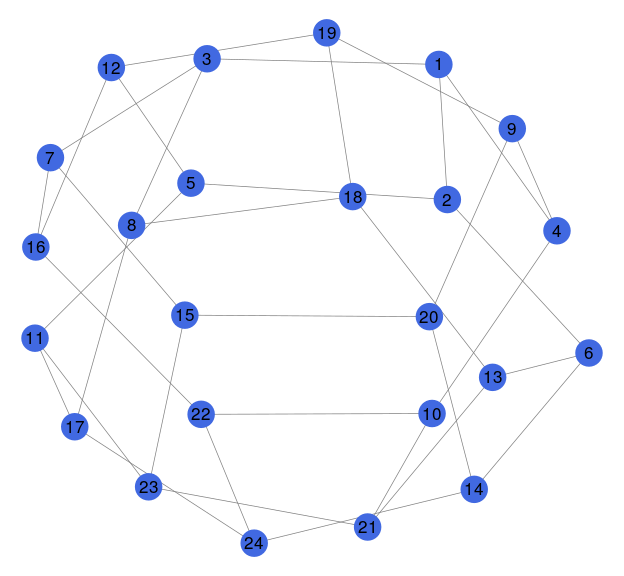
\includegraphics[width=0.7\linewidth]{week02_files/figure-latex/fig:cycle-diam-1} 

}

\caption{命題の反例}\label{fig:fig:cycle-diam}
\end{figure}

girthとdiameter

\begin{Shaded}
\begin{Highlighting}[]
\NormalTok{iG =}\StringTok{ }\KeywordTok{read_graph}\NormalTok{(}\StringTok{'../resource/graph/n14-d3-nogmg.elist'}\NormalTok{)}
\KeywordTok{paste}\NormalTok{(}\KeywordTok{girth}\NormalTok{(iG)}\OperatorTok{$}\NormalTok{girth, }\KeywordTok{diameter}\NormalTok{(iG))}
\end{Highlighting}
\end{Shaded}

\begin{verbatim}
## [1] "5 3"
\end{verbatim}

\section*{参考文献}
\addcontentsline{toc}{section}{参考文献}

\hypertarget{refs}{}
\hypertarget{ref-Cerf1974}{}
{[}1{]} V. G. Cerf, D. D. Cowan, R. C. Mullin, and R. G. Stanton,
Networks \textbf{4}, 335 (1974).

\hypertarget{ref-Yamamoto2016}{}
{[}2{]} 山本康. and 高橋規., (2016).


\end{document}
